\documentclass[../rapport.tex]{subfiles}
\graphicspath{{\subfix{ressources/photos_diagrammes/extensionThomas/}}}

\begin{document}
		\subsubsection{Vue d'ensemble}
		Le but de cette extension est de rajouter la gestion de contrats d'assurances divers
		à la fois pour les client smais égalemet pour les insitutions. L'extension se base tout
		de même sur la structure de l'application 1 car c'est dans celle-ci qu'elle la plus 
		utilisée. En effet, dans l'appliction 2 elle est gére comme les autres produits 
		financiers. Il n'y a réellement que la réponse à une demande de devis qui diffère.
		Afin de rendre les diagrammes plus visibles j'ai changé les couleurs des éléments rajoutés. 
		Rose pour le diagramme d'entité relation et jaune pour les autres diagrammes.

		\subsubsection{Application 1}

		\subsubsection{Diagramme des cas d'utilisation}
				\begin{figure}[h]
						\centering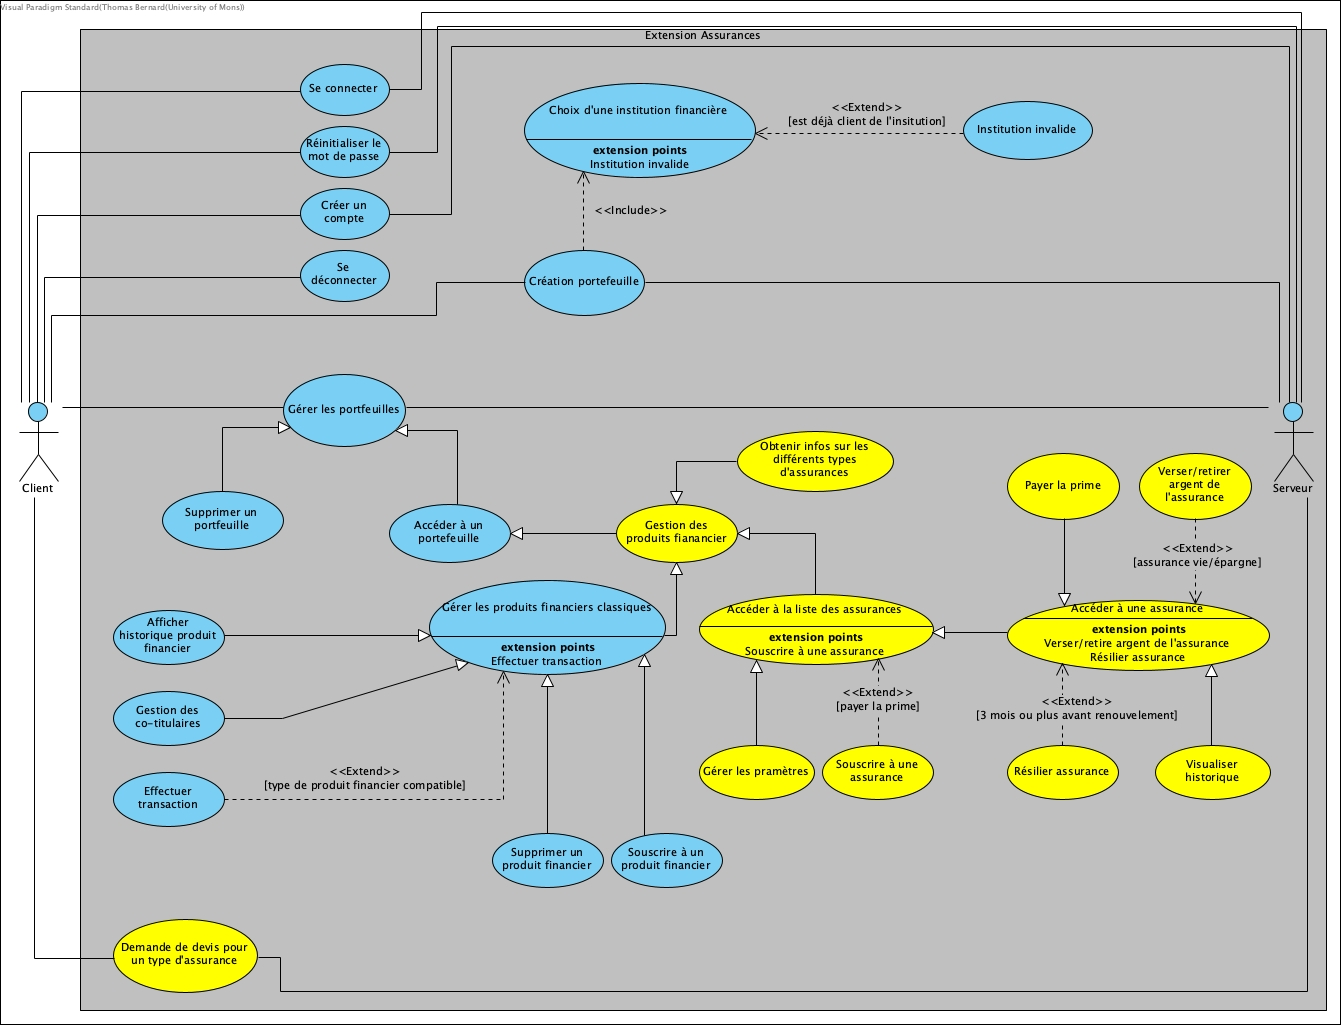
\includegraphics[scale=0.27]{ressources/photos_diagrammes/extensionThomas/useCase1Thomas.jpg}
						\caption{Diagramme des cas d'utilisation de l'app 1 avec extension}
				\end{figure}
		J'ai rajouté un ensemble de divers cas d'utilisations qui sont propres aux assurances
		mais toutefois semblables aux cas d'utilisation relatifs aux produits financiers
		classiques. Il n'y a aucune remarque particulière à faire concernant les cas
		d'utilisation car le modèle est calqué sur le diagramme de base.
\newpage
		\subsubsection{Interaction Overview Diagram}
				\begin{figure}[h]
						\centering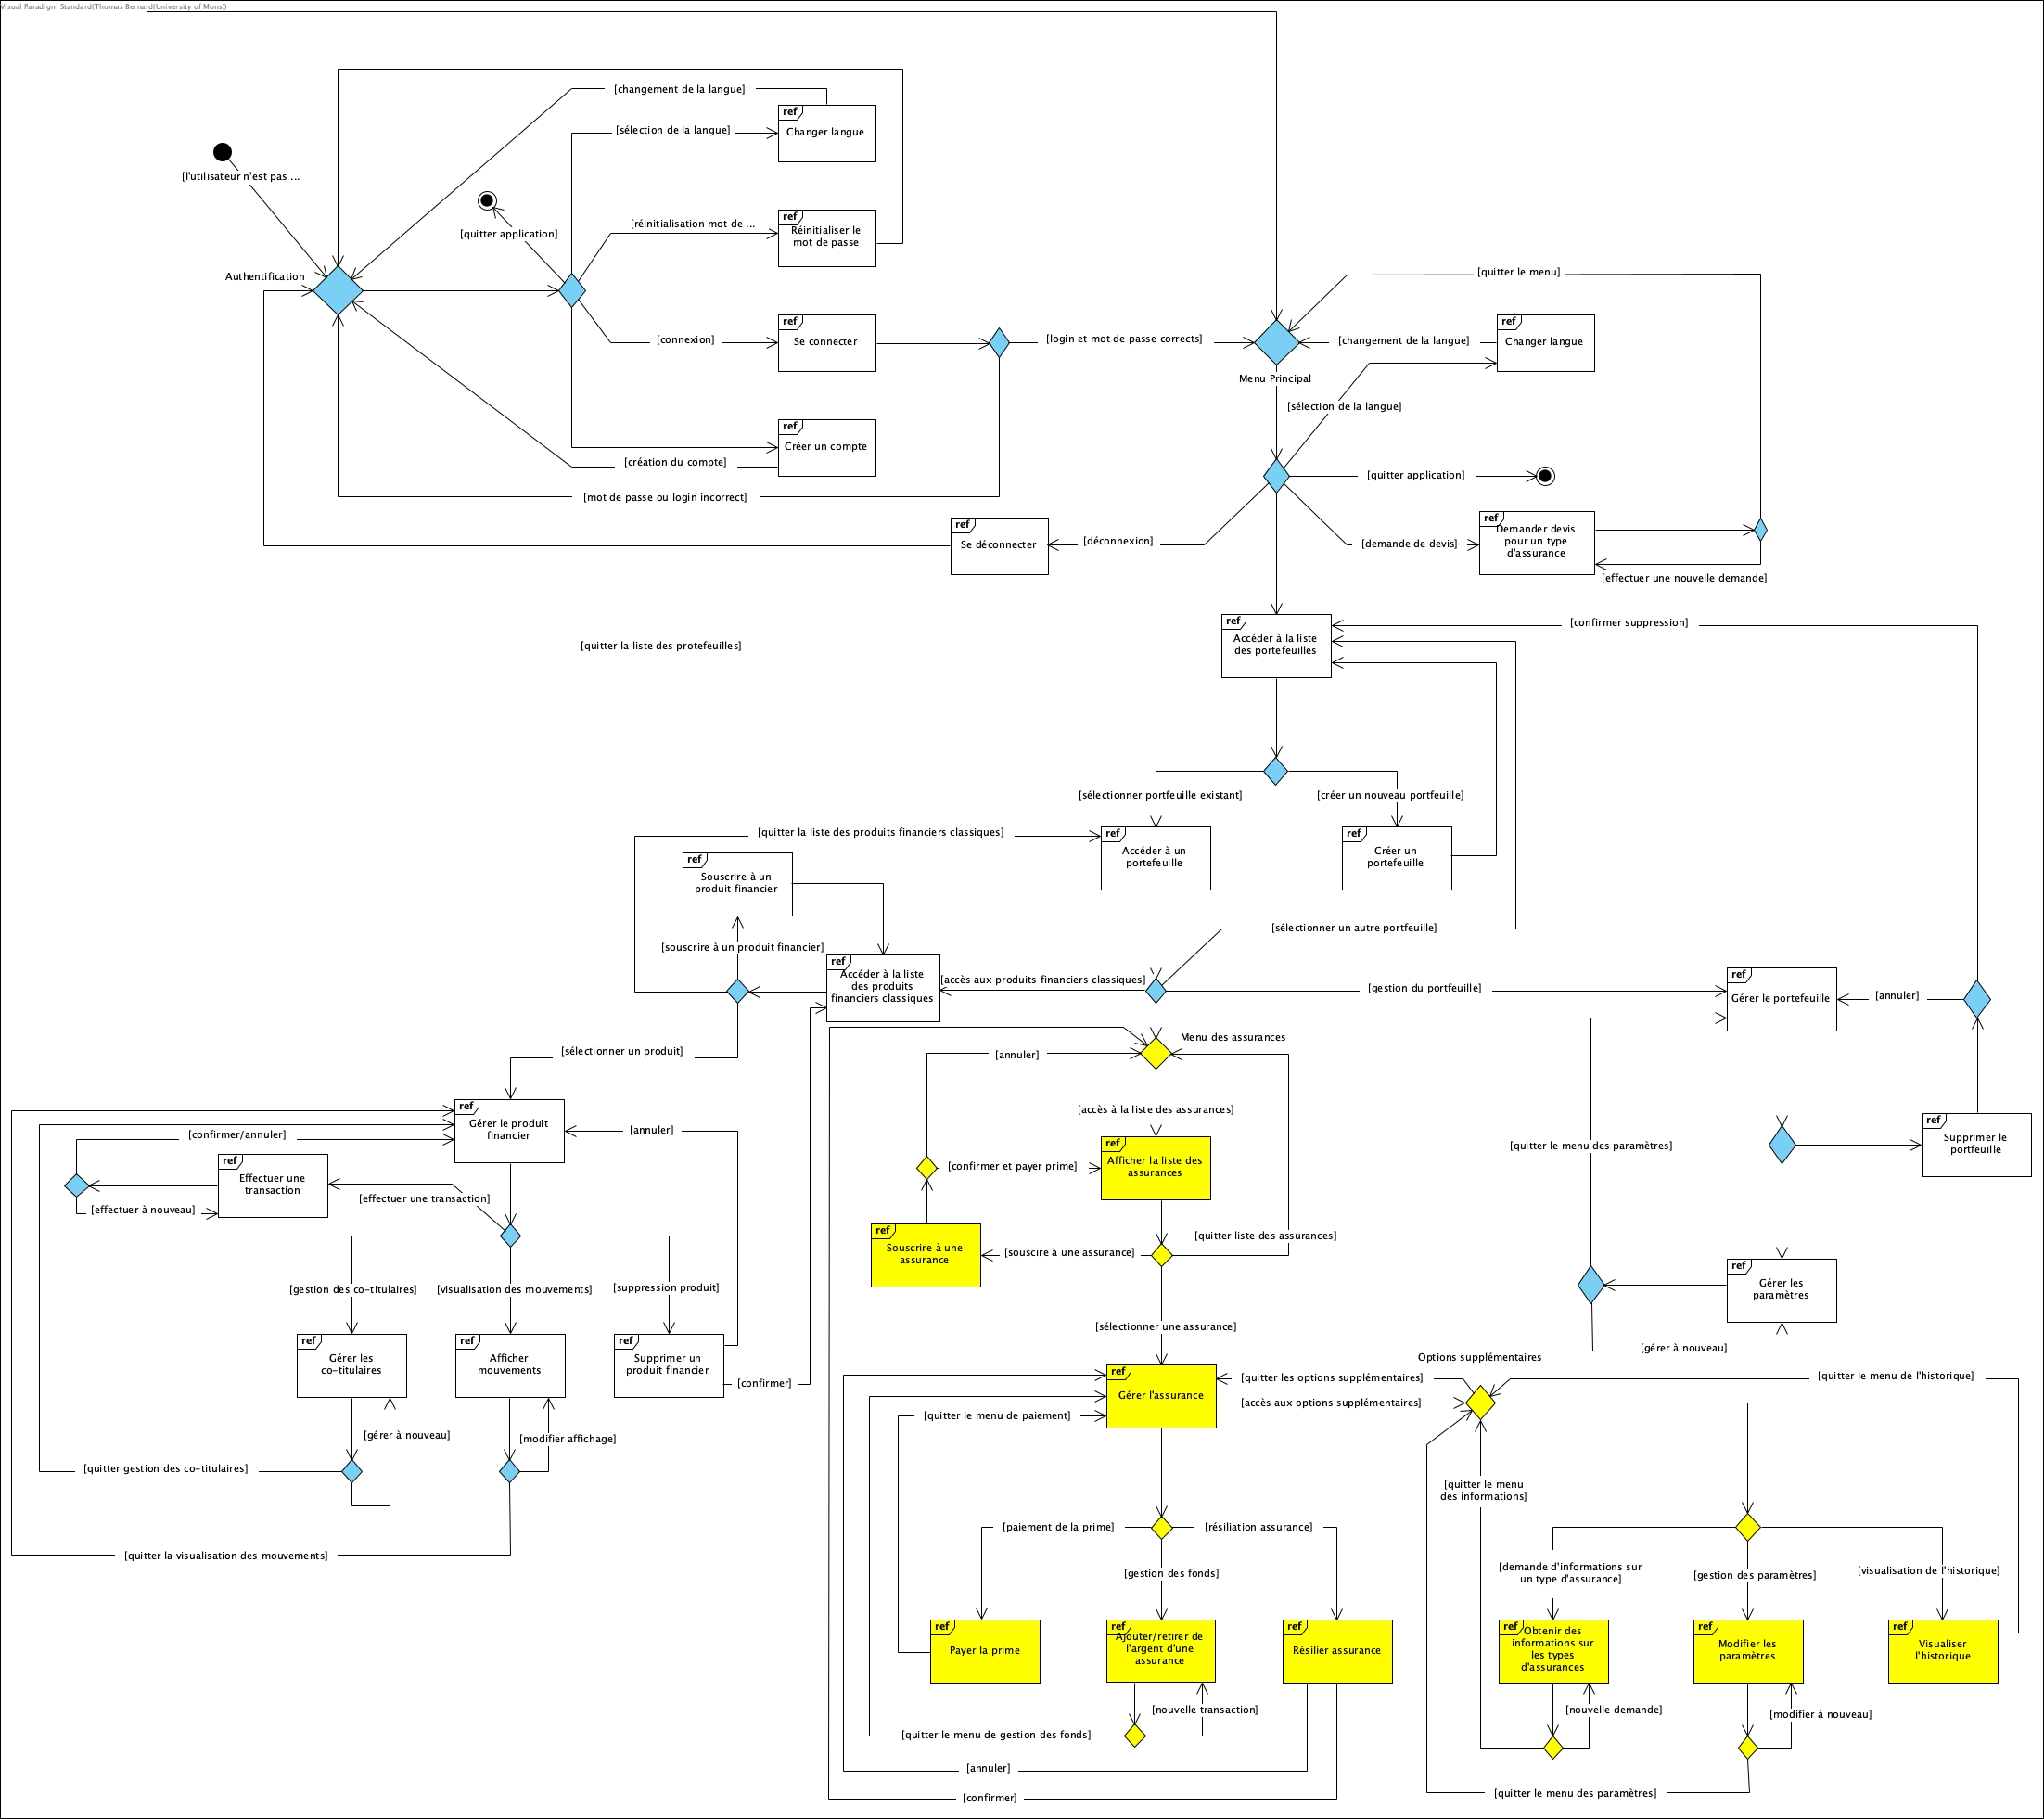
\includegraphics[scale=0.15]{ressources/photos_diagrammes/extensionThomas/intOver1Thomas.jpg}
						\caption{Interaction Overview Diagram de l'app 1 avec extension}
				\end{figure}
		Encore une fois ce diagramme se base sur celui de l'application 1. Notons qu'il est
		maintenant possible de demander un devis depuis le menu principal. Il y a également une 
		différenciation entre les produits financiers classiques et les assurances afin de les 
		séparer en deux scènes différentes plus tard dans la GUI.

\newpage
		\subsubsection{Diagrammes de classe}
				\begin{figure}[h]
						\centering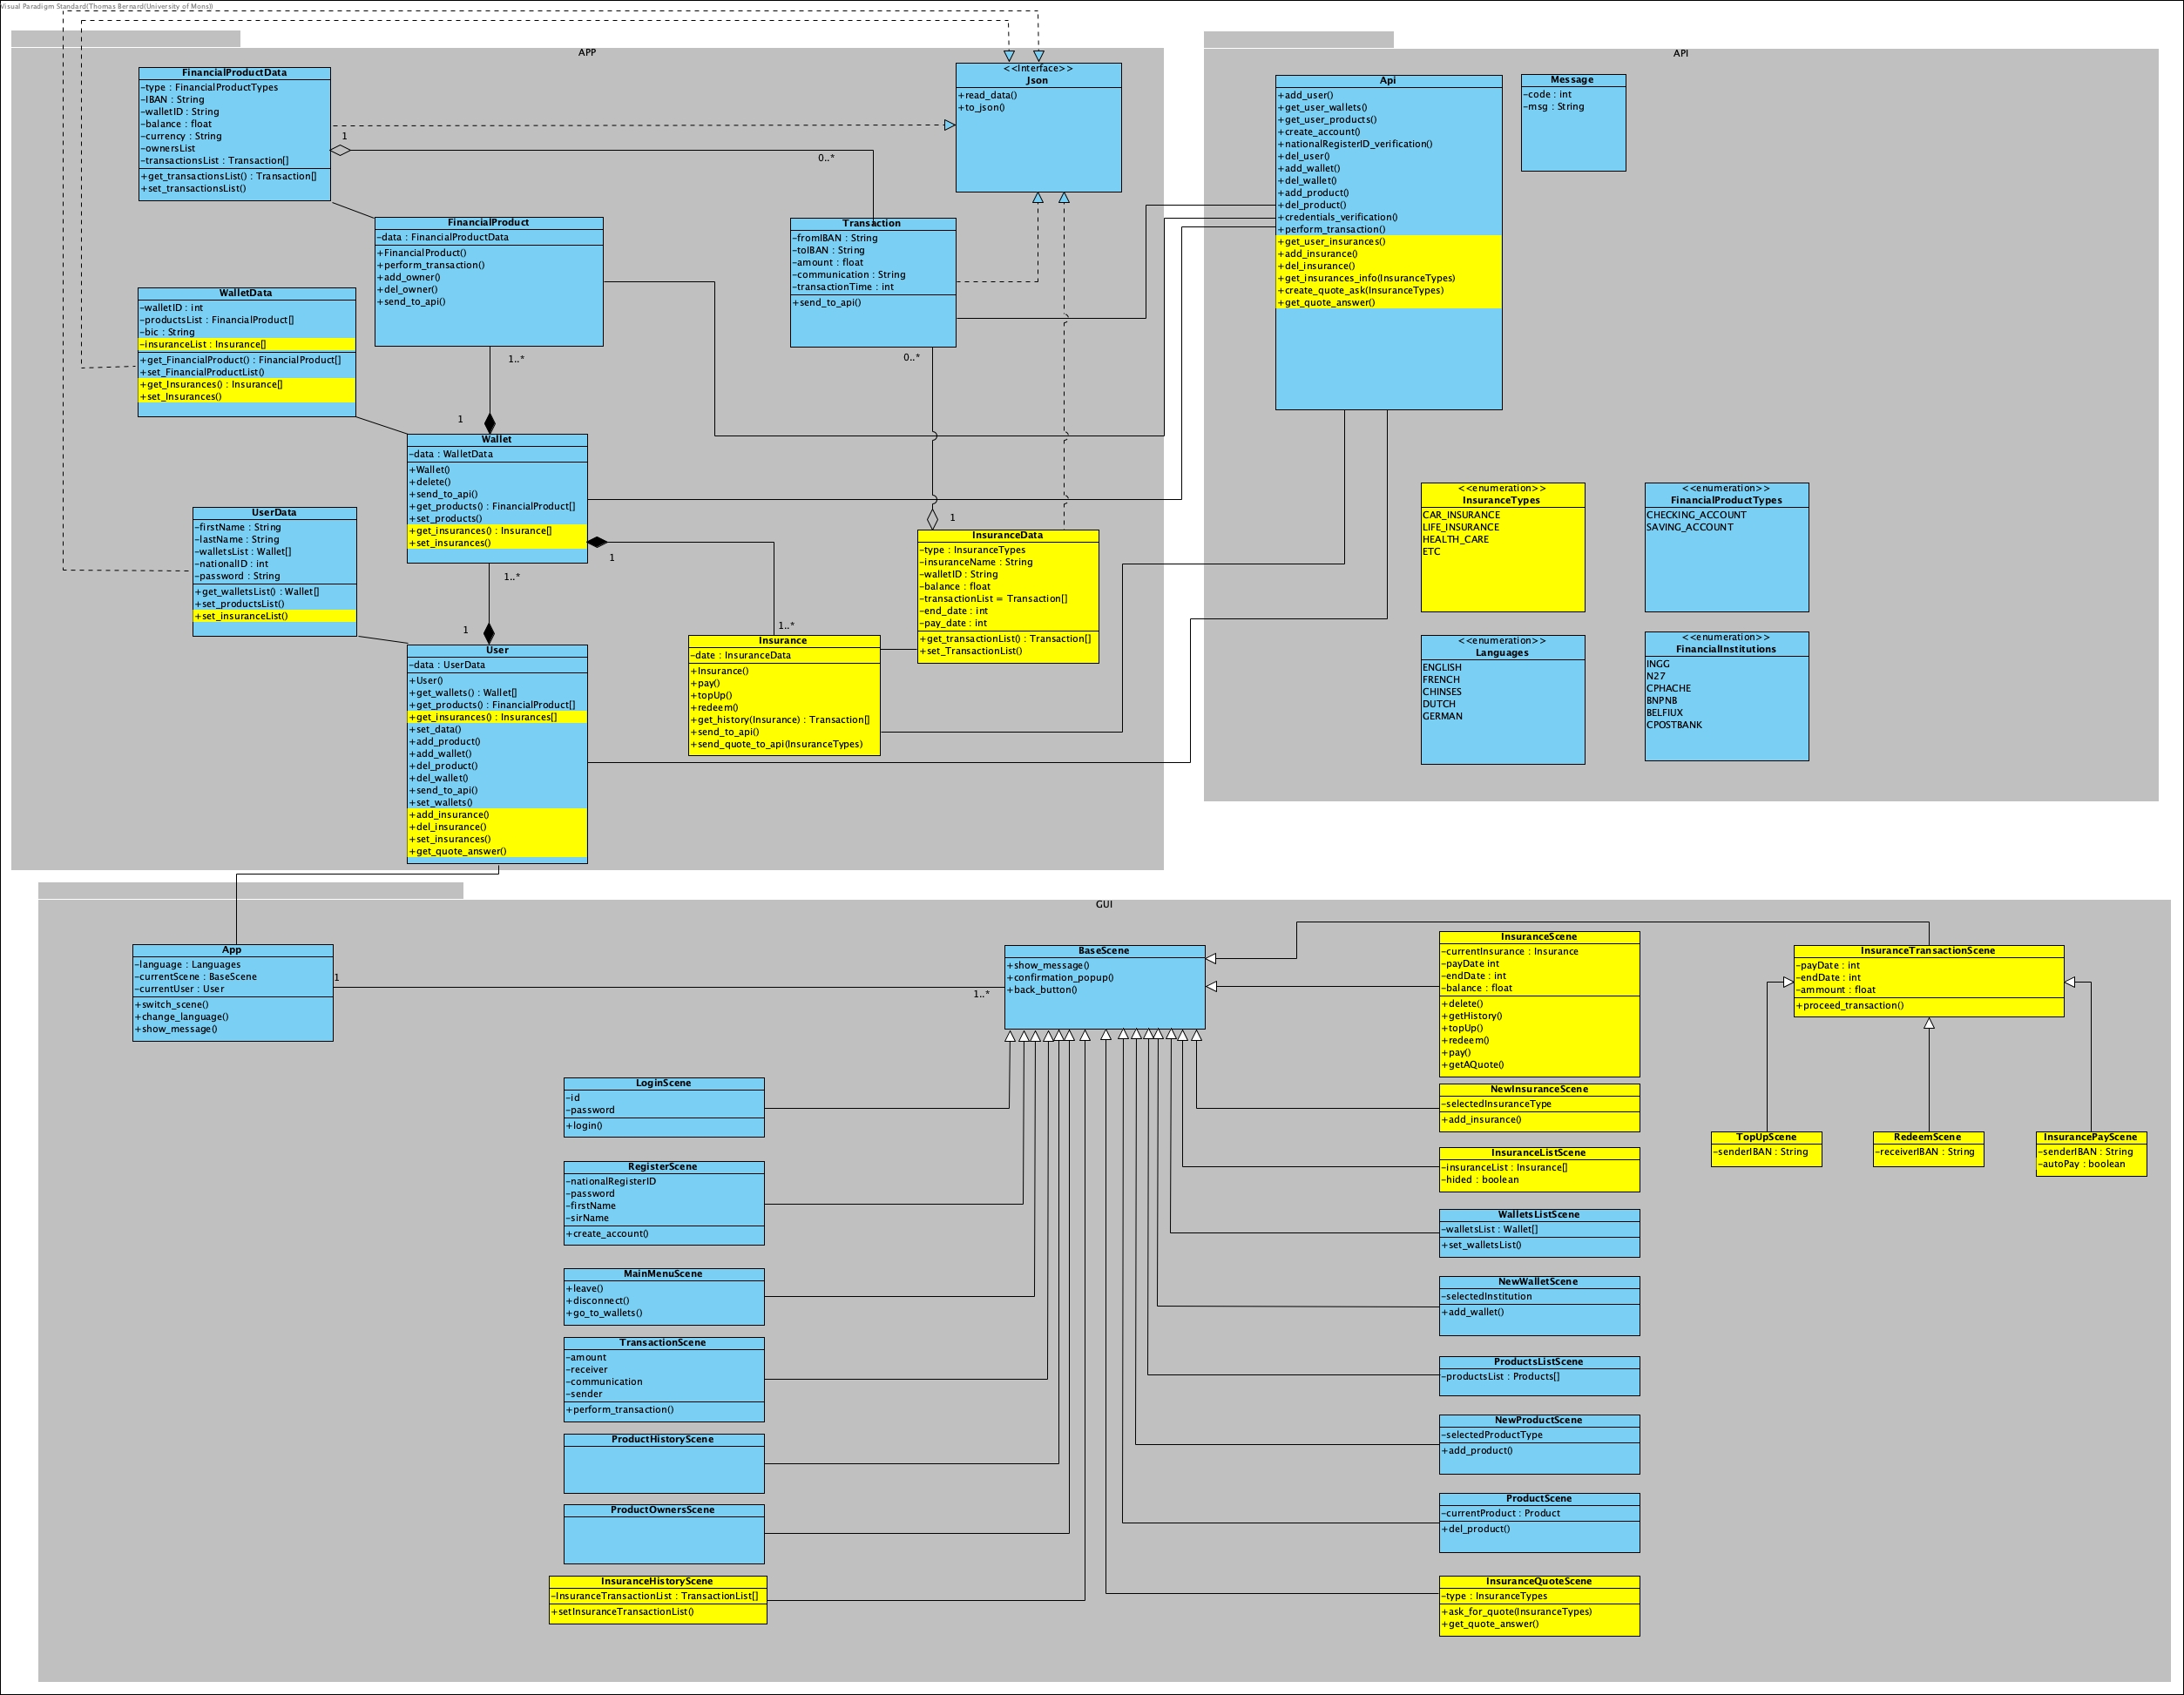
\includegraphics[scale=0.15]{ressources/photos_diagrammes/extensionThomas/classes1Thomas.jpg}
						\caption{Diagramme de classes de l'app 1 avec extension}
				\end{figure}
		Dans la partie logique de l'application (package APP) deux classes ont été rajoutées :
		\textbf{Insurance} et \textbf{InsuranceData}. La première contioent le constructeur et 
		un attribut \textit{data} qui est une objet de type \textit{InsuranceData}. La classe 
		contient également les méthodes liées aux assurances. La classe \textbf{Insurance} est
		liée à la classe wallet de même manière que la classe \textbf{FinancialProduct}. 
		La classe \textbf{Insurance} possède une méthode \textit{send\_to\_api()} et est connectée 
		au package API. La classe \textbf{InsuranceData} implémente l'interface \textbf{Json} qui
		permet d'écrire et le dire des fichiers :json de données et d'ainsir mettre ses données à
		jour.

		\medskip

		Les classes de bases dans lesquelles se trouvaient des listes de produits, des setter et 
		des getter se sont vues ajouter des setter, des getter et des listes mais cette fois-ci
		pour les assurances. 

		\bigskip

		Dans la partie serveur du diagramme de classe (package API) j'ai rajouté une enumération
		\textbf{InsurancesTypes} qui contient les différents types d'assurances afin de pouvoir
		interpréter correctment les données envoyées à la classe \textbf{Api}. Dans la classe
		\textbf{Api} des méthodes ont été rajoutées afin de pouvoir ajouter, supprimer et obtenir
		les assurances d'un client. Il y a également une méthode permettant d'obtenir des 
		informations sur un ou plusieurs types d'assurances dans le cadre de devis.

		\bigskip

		Dans la partie interface graphique (package GUI) il s'agit principalement de nouvelles 
		scènes rajoutées à la manière des scènes de l'application de base. Il n'y a pas de 
		point particulier à expliquer ici.
		
		\subsubsection{Diagrammes de séquence}
				\paragraph{Souscrire à une assurance :}
						\begin{figure}[h!]
								\centering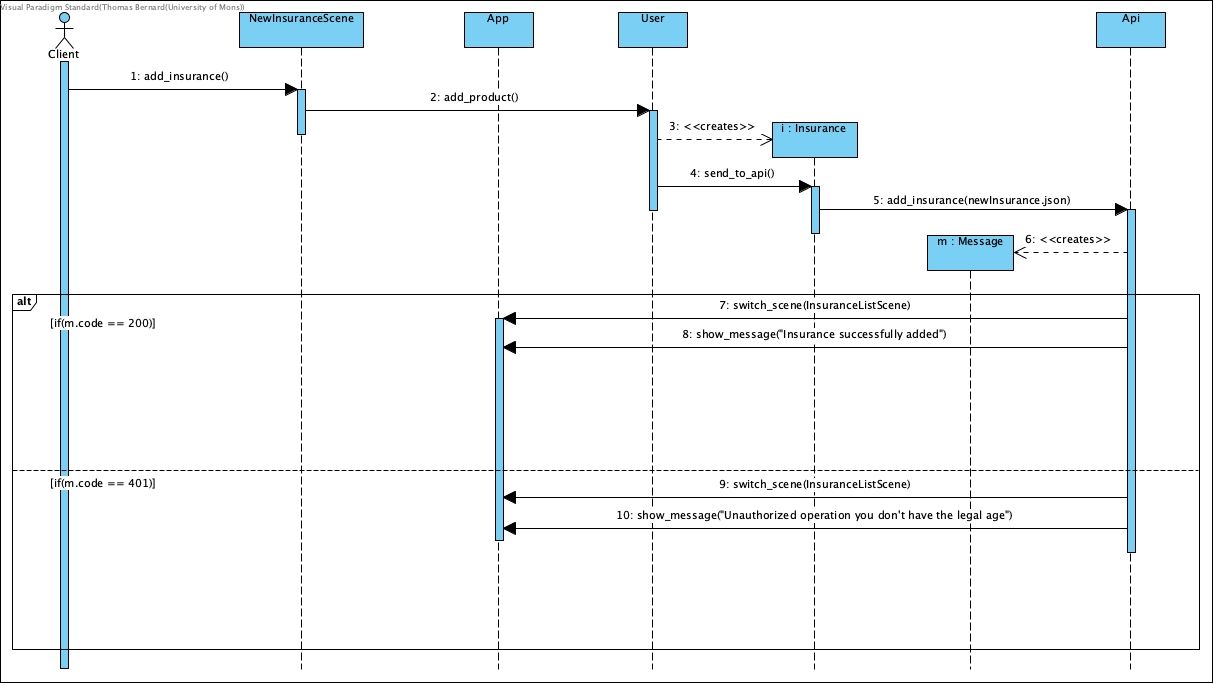
\includegraphics[scale=0.3]{ressources/photos_diagrammes/extensionThomas/souscrireAssurance.jpg}
								\caption{Souscrire à une assurance}
						\end{figure}
					Lorsque le client souhaite souscrire à une assurance l'application envoie à l'API une reqûete contenant les informations du demandeur ainsi que les informations de l'assurance
					demandée. L'API ajoute l'assurance à la base de données. Si l'ajout a bien eu lieu alors la scène change sur celle de la liste des assurances qui lors de sa création récupère
					les assurances du client. L'application affiche le message qui dit que l'assurance a bien été ajoutée.
					\medskip
					Si l'ajout n'a pas lieu le client est redirigé sur la scène de la liste des assurances et un message l'informe de l'erreur.
\newpage
				\paragraph{Afficher la liste des assurances :}
						\begin{figure}[h!]
								\centering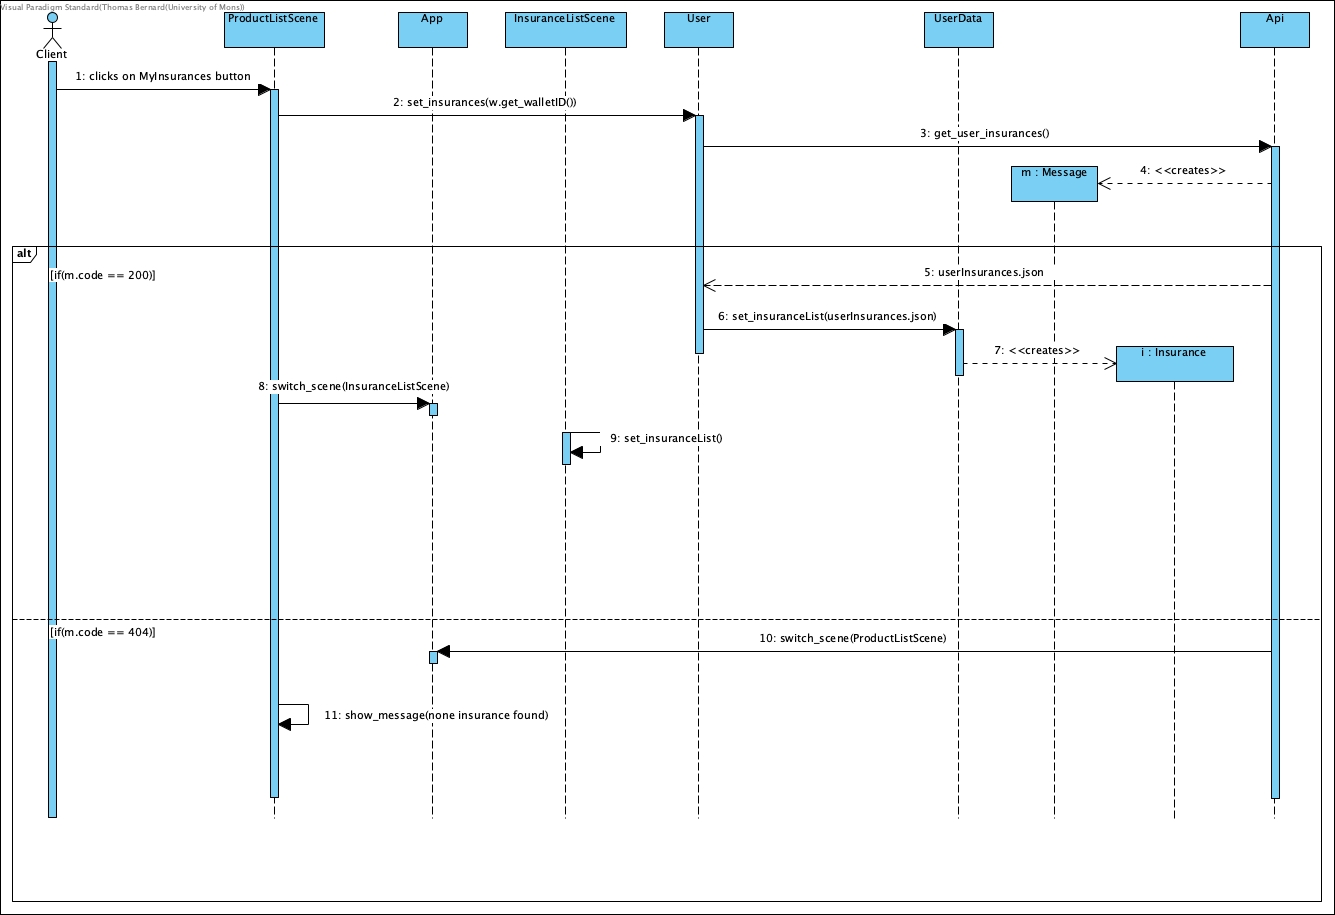
\includegraphics[scale=0.3]{ressources/photos_diagrammes/extensionThomas/afficherListeAssurances.jpg}
								\caption{Afficher la liste des assurances}
						\end{figure}
						
					Lorsque le client souhaite accéder à la liste de ses assurance une requête contenant le wallet et le userID du client est envoyée à l'API afin 
					que celle-ci renvoie la liste des assurances. Il ya 2 réponses possible. Soit l'API trouve des assurances, met à jour la liste dans l'application
					Lorsque l'application change la scène pour afficher la InsuranceListScene la scène est instanciée et la liste est mise à jour à l'aide du fichier 
					Json renvoyé par l'API. 
					Sinon l'API renvoie une erreur. L'application change la scène sur la ProductListScene et informe le client qu'aucune assurance n'a été trouvée.
\newpage		

				\paragraph{Ajouter/retirer de l'argent d'une assurance}

						\begin{figure}[h]
								\centering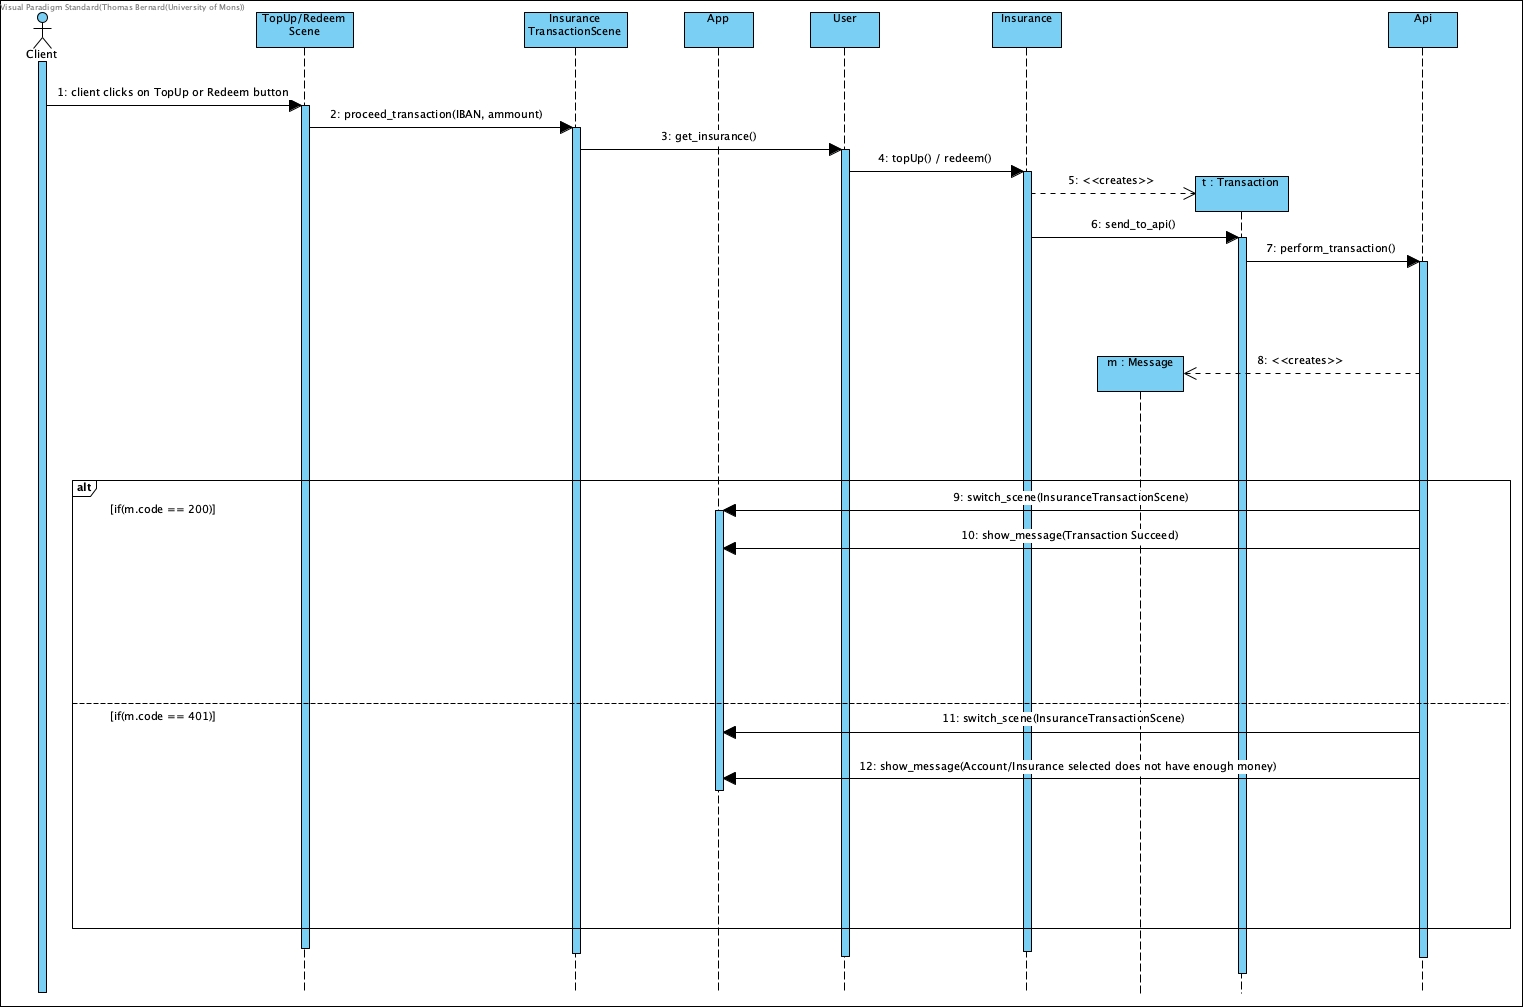
\includegraphics[scale=0.25]{ressources/photos_diagrammes/extensionThomas/ajoutRetraitAssurance.jpg}
								\caption{Ajouter/retirer de l'argent d'une assurance} 
						\end{figure}

						Lorsque le client souhaite ajouter/retirer de l'argent d'une assurance une requête est envpoyée à l'API contenant le compte sur lequel il faut 
						ajouter/retirer de l'argent ainsi que l'assurance courrante. Il y a 2 types de réponses possibles. Soit tout se passe bien et l'API renvoie un
						message success à l'application. Dans ce cas l'application renvoie le client sur la InsuranceTransactionScene et met à jour les comptes ainsi 
						que l'assurance. 
						\medskip

						Soit l'API renvoie un message d'erreur à l'application. Dans ce cas l'application renvoie le client sur la InsuranceTransactionScene et l'informe
						que le compte/assurance sélectionné pour l'ajout/retrait ne possède pas un solde suffisament élevé et lui dit changer de compte ou de 
						l'approvisionner avant de réitérer l'opération.

\newpage 
				\paragraph{Payer la prime d'une assurance}

						\begin{figure}[h]
								\centering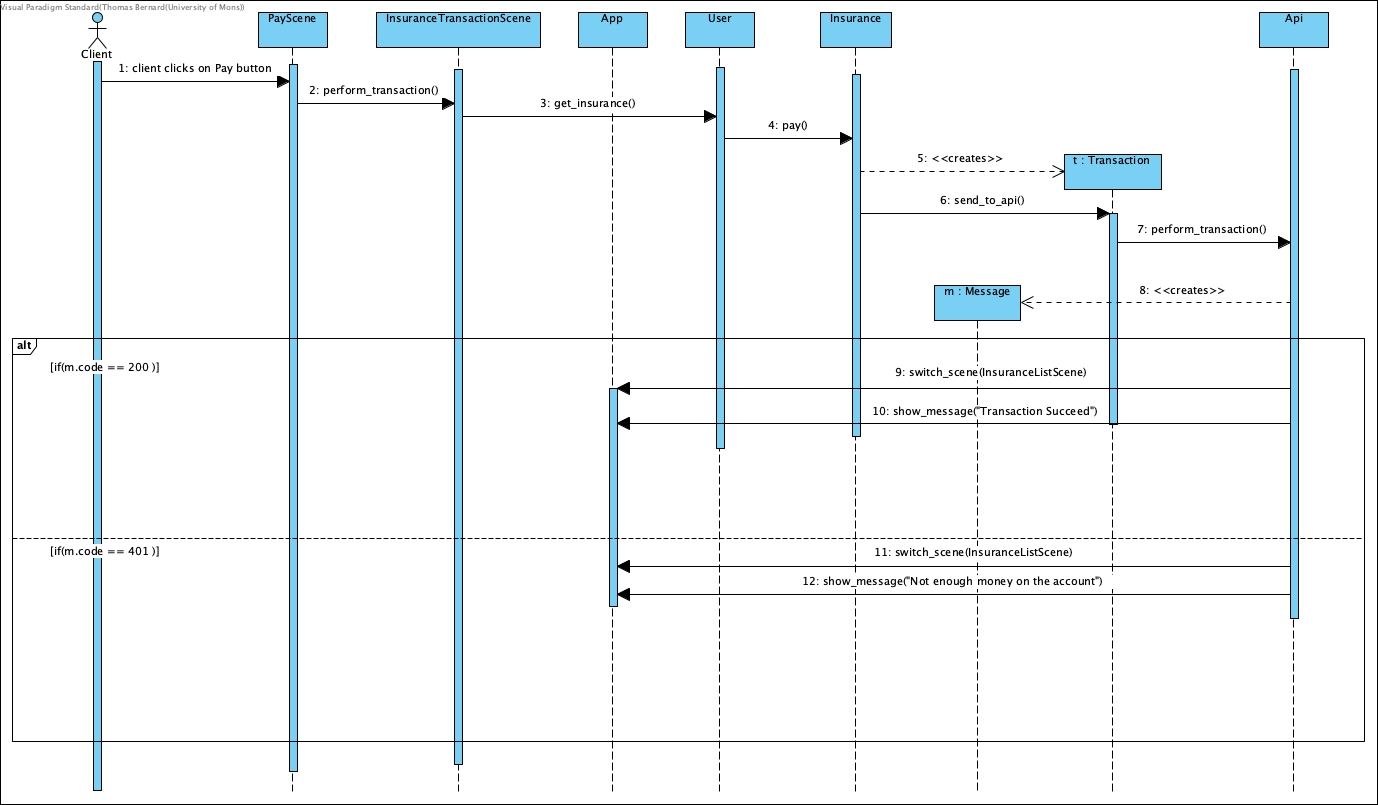
\includegraphics[scale=0.3]{ressources/photos_diagrammes/extensionThomas/payerLaPrime.jpg}
								\caption{Payer la prime de l'assurance}
						\end{figure}

						Lorsque le client souhaite payer la prime une requête contenant l'assurance en question ainsi que le montant et le compte à débiter est envoyée
						à l'API. Deux résulats sont possibles. Soit le solde du compte est suffisant et l'API renvoie un message de succès qui est affiché par
						l'application lorsqu'elle renvoie l'utilisateur dans la InsuranceListScene. Soit le solde est insuffisant et un message d'erreur est envoyé 
						sur cette même scène à l'utilisateur lui demande de sélectionner un autre compte ou bien de l'approvisionner.

\newpage

				\paragraph{Effectuer une demande de devis}

						\begin{figure}[h]
								\centering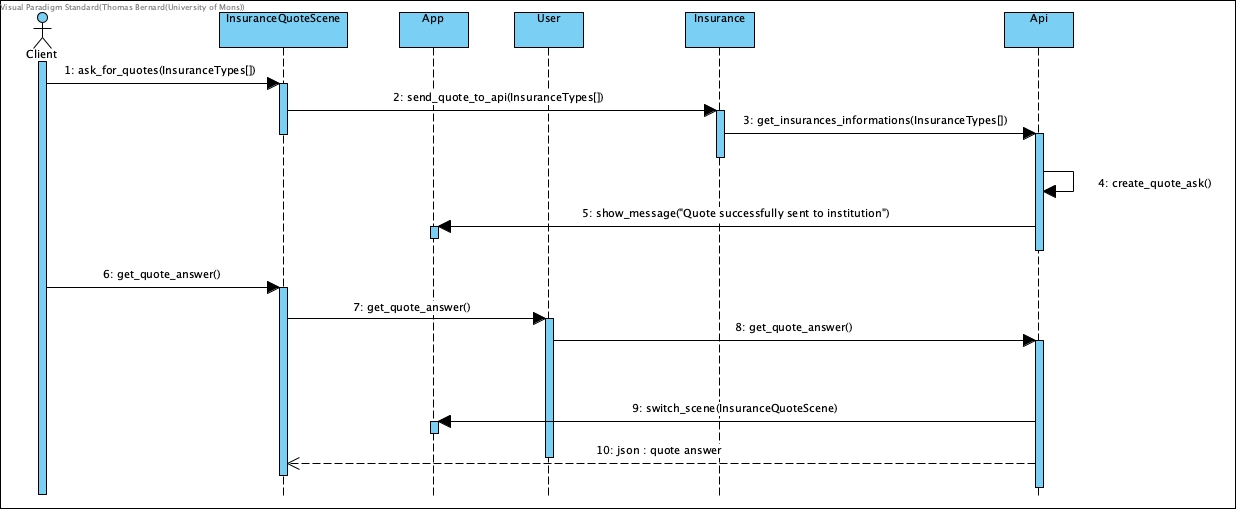
\includegraphics[scale=0.3]{ressources/photos_diagrammes/extensionThomas/demanderDevis.jpg}
								\caption{Effectuer une demande de devis}
						\end{figure}
						Lorsque le client effectue une demande de devis une requête contenant un type d'assurance est envoyée à l'API cette reqûete est traduite en un ajout
						dans la base de données par l'API qui ajoute la demande dans une table dédiée à cette utilisation. Ensuite l'API renvoie un message qui est affiché
						par l'application et qui informe l'utilisateur que sa demande a bien été envoyée à l'institution. 

						L'utilisateur peut également contrôler s'il a reçu une réponse dans ce cas on appelle une méthode dans l'API afin de contrôler s'il y a une réponse.
						L'API renvoie le devis au travers d'un fichier Json qui est interprété par l'application et affiché à l'utilisateur.
\newpage

		\subsubsection{Application 2}

		\subsubsection{Diagramme des cas d'utilisitation}

				\begin{figure}[h]
						\center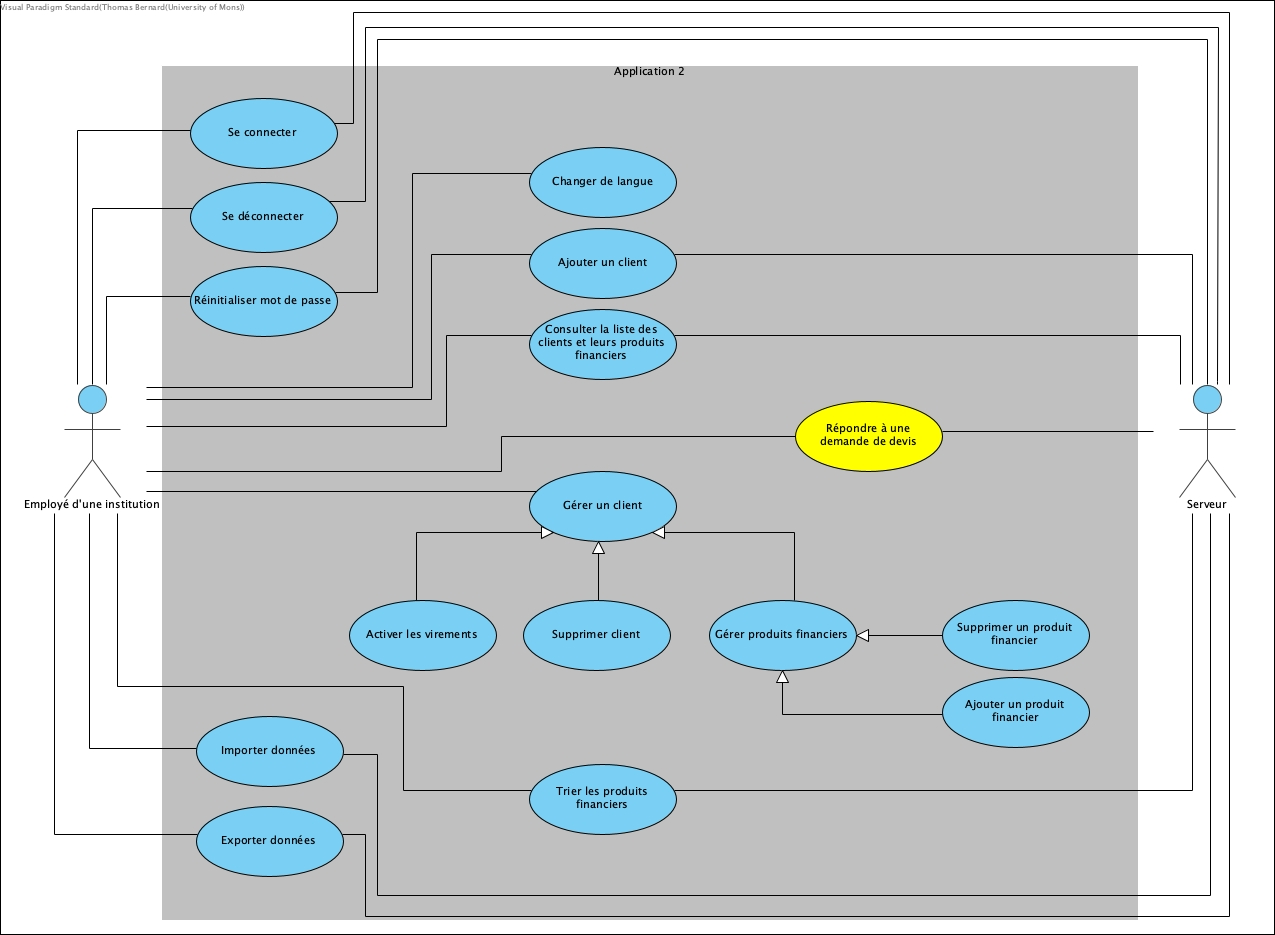
\includegraphics[scale=0.27]{ressources/photos_diagrammes/extensionThomas/useCase2Thomas.jpg}
						\caption{Diagramme des cas d'utilisation de l'app 2 avec extension}
				\end{figure}

				Le diagramme de cas d'utilisation de l'app 2 ne contient qu'une seule modification.
				Il s'agit du use case permettant de répondre à un devis. En effet lorsqu'une
				institution liste les produits d'un client elle liste également ses assurances.
				Il n'est donc pas nécessaire d'ne rajouter plus.

		\subsubsection{Interaction Overview Diagram}

		Il n'y a également qu'un seul cas d'utilisation rajouté qui est celui de réponse à un
		devis. Par souci de taille du diagramme il n'a pas été ajouté au rapport. L'interaction
		a été rajoutée au niveau du menu de gestion des clients. Une fois l'utilisation terminée,
		le user de l'institution est ramené vers le menu des produits.

		\subsubsection{Diagramme de classes}

				\begin{figure}[h]
						\centering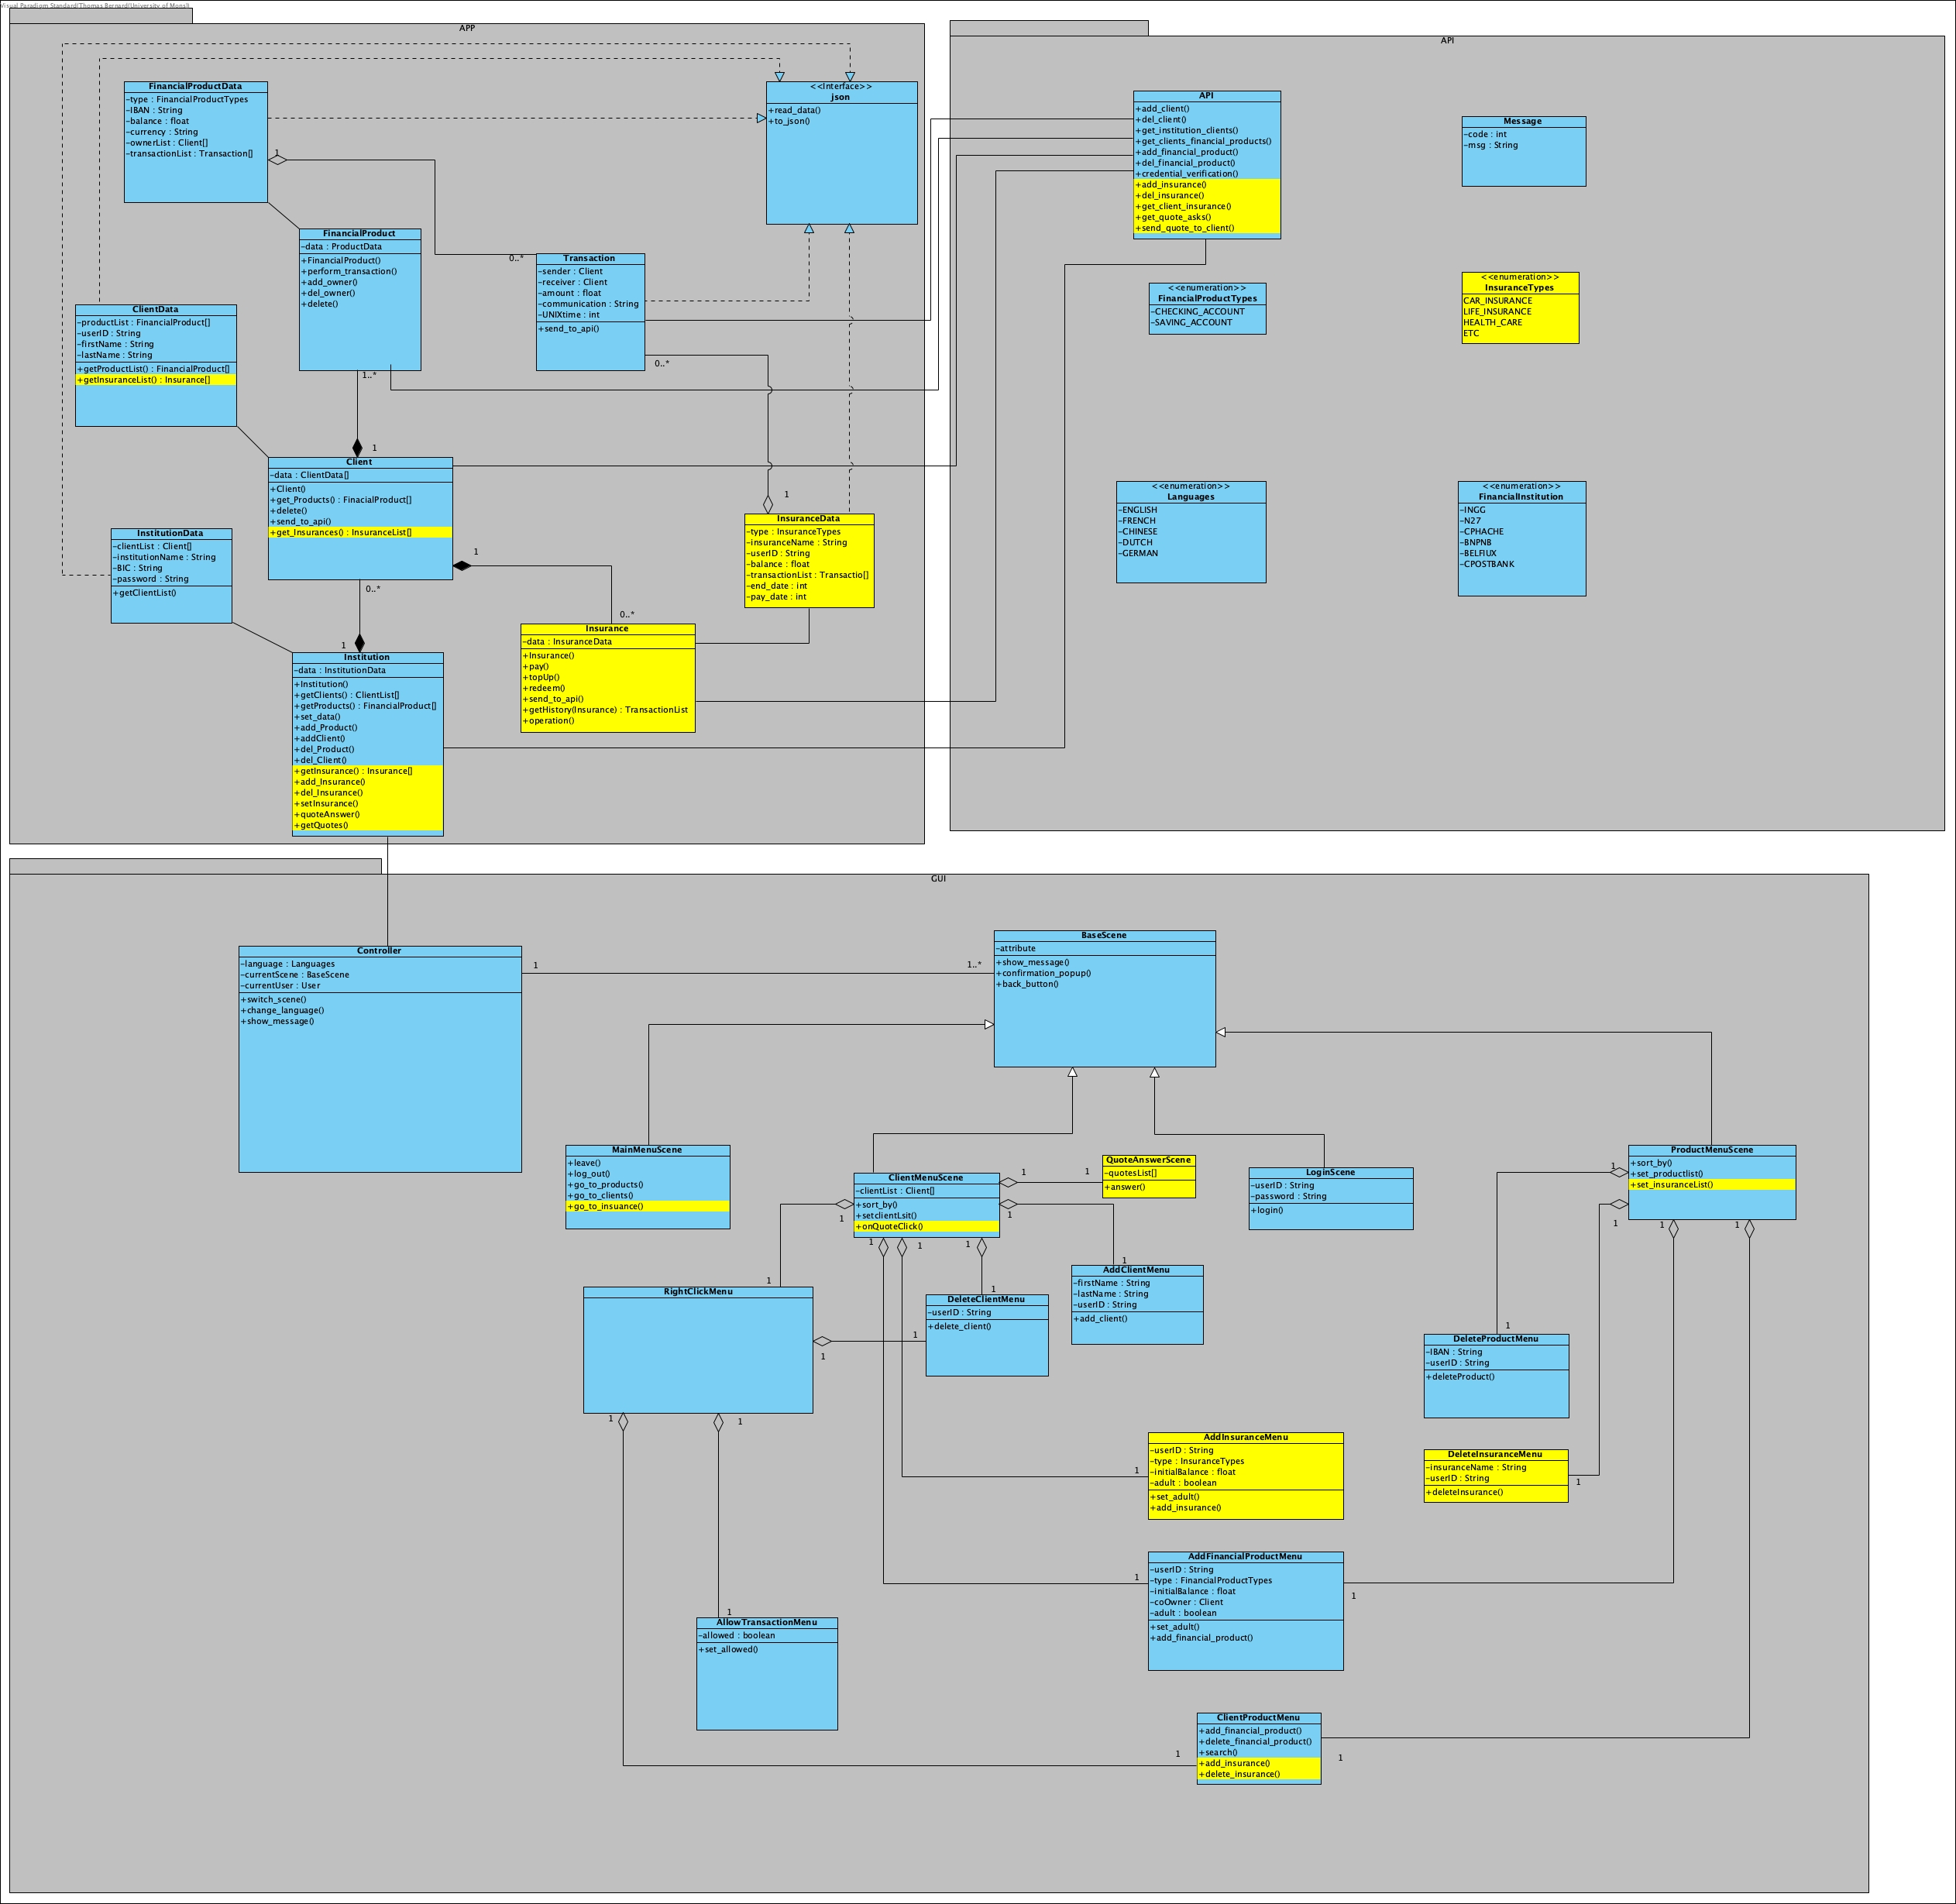
\includegraphics[scale=0.15]{ressources/photos_diagrammes/extensionThomas/classes2Thomas.jpg}
				\end{figure}
		Au niveau de la logique de l'application (package APP) mise à part le fait que la classe 
		\textbf{Insurance} est maintenant reliée à la classe \textbf{Client} du fait que les 
		instituions n'aient pas la notion de portfeuilles et qu'une méthode \textit{quoteAnswer()}
		ait été rajoutée à la classe \textbf{Institution} permettant d'envoyer le devis au client,
		il n'y a pas de changements importants par rapport à celui de l'application 1. 

		\bigskip

		Au niveau de la partie serveur de l'application (package API) le seul cahnegement à noter
		est l'ajout d'une méthode \textit{answerQuote()} dans la classe \textbf{Api} qui permet
		à l'API de générer des réponses à une demande de devis.

		\bigskip

		Au niveau de la partie interface graphique de l'application (package GUI). Une méthode 
		permettant d'accéder à la scène liée aux assurances a été ajoutée à la classe 
		\textbf{MainMenuScene} et une méthode permettant d'accéder à la scène de demande des devis
		a été ajoutée dans la classe \textbf{ClientMenuScene}. Enfin une méthode permettant 
		d'afficher les assurances des clients a été ajoutée à la classe \textbf{ProductMenuScene}.

		\medskip

		Pour ce qui est des classes ajoutées, elles sont au nombre de 3.\\
		Il s'agit des classes suivantes :
		\begin{enumerate}
				\item \textbf{QuoteAnswerScene:} qui est la scène où toutes les demandes de devis
						sont listées et qui contient un bouton permettant d'y répondre.
				\item \textbf{AddInsuranceMenu} cette scène permet d'ajouter une assurance pour
						un client en particulier
		\end{enumerate} 
\newpage
		\subsubsection{Diagrammes de séquences}
				\begin{figure}[h]
						\centering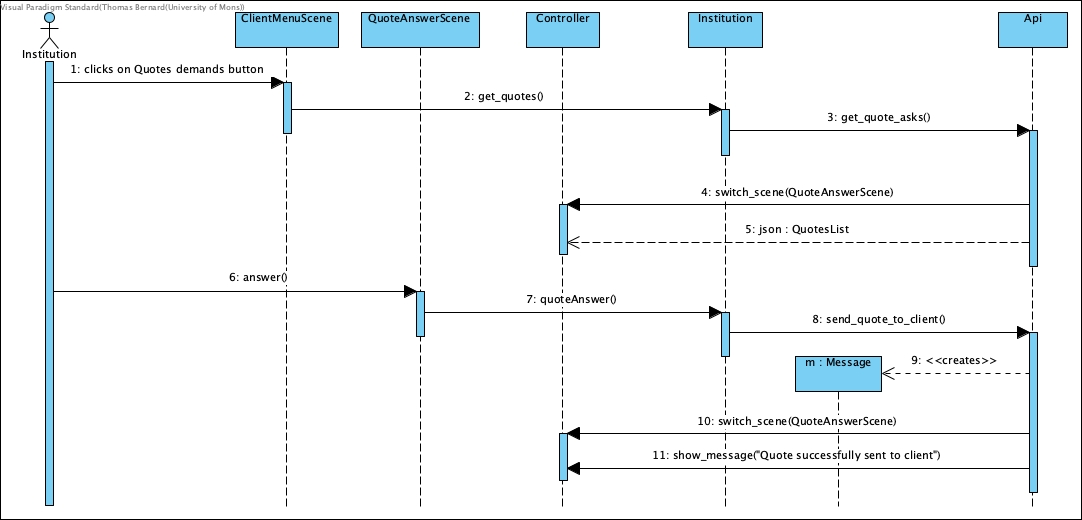
\includegraphics[scale=0.3]{ressources/photos_diagrammes/extensionThomas/reponseDevis.jpg}
						\caption{Réponse à une demande de devis}
				\end{figure}

				L'insitution lorsque décide d'accèder à la scène des demande devis envoie une
				reqûete à l'API qui va rechercher la liste des demandes de devis qui sont propres
				à l'institution dans la base de données. Ainsi quand la scène est affichée la 
				liste l'est également. Lorsque que l'insitution appuie sur answer une requête est
				envoyée à l'API qui va chercher les informations liées au type d'assurance demandé
				par le client et le stocke dans la base de données.
		\subsubsection{Serveur}
		\subsubsection{Diagramme d'entité relation}

				\begin{figure}[h]
						\centering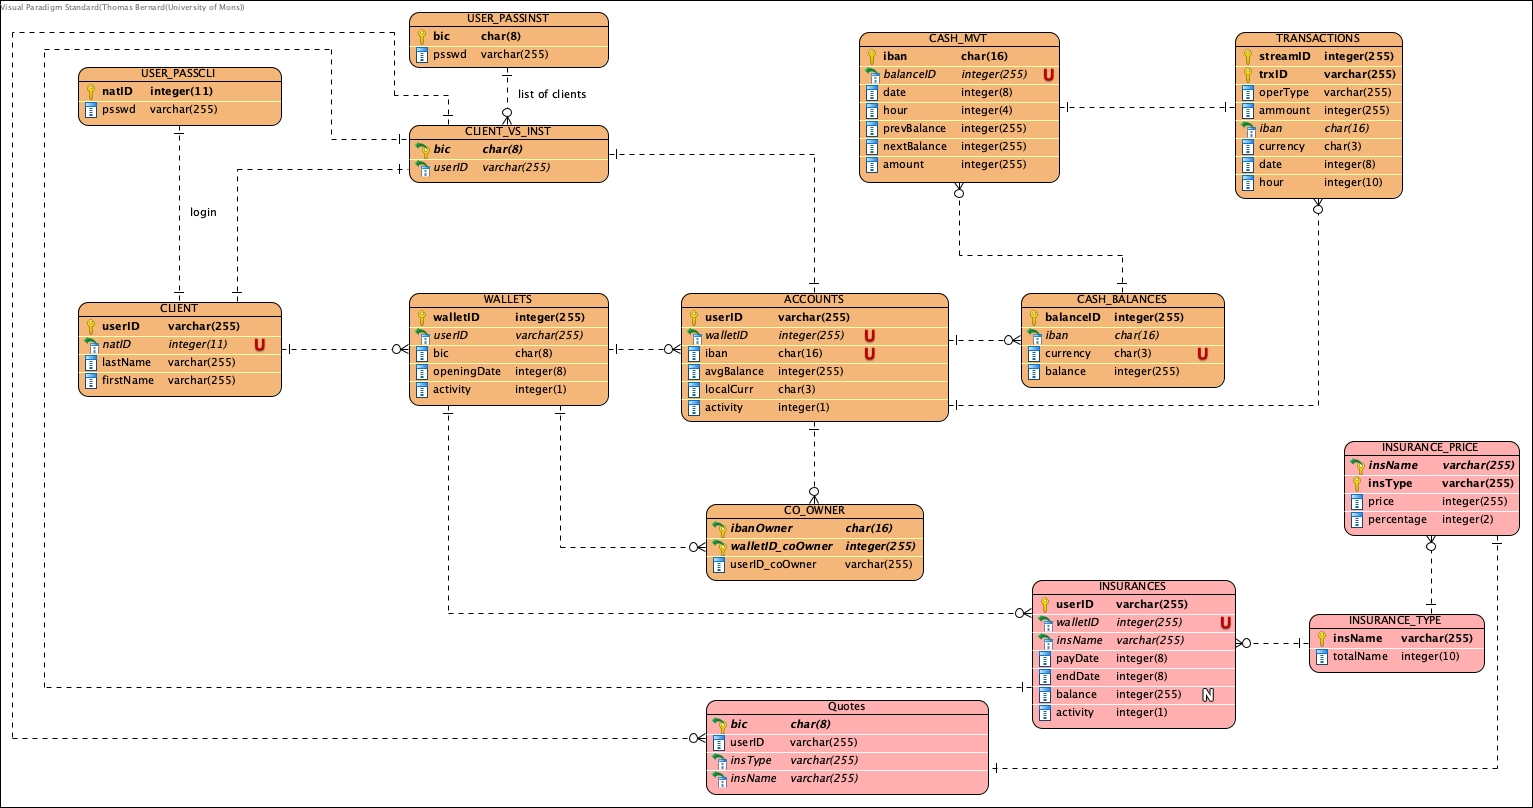
\includegraphics[scale=0.25]{ressources/photos_diagrammes/extensionThomas/erdThomas.jpg}
						\caption{Diagramme d'entité relation avec extension}
				\end{figure}
		Le diagramme d'entité relation a été étendu à l'aide de 3 tables : \textit{INSURANCES, ISNURANCE\_TYPE et INSURANCE\_PRICE}.
				
		\medskip

		La table \textit{INSURANCES} contient toutes les assurances des clients. Elle peut être accédée par 2 tables : par la table \textit{WALLETS} grâce au walletID qui lui est lié dans le cadre de l'application client et par la table \textit{CLIENT\_VS\_INST} grâce au userID qui est lié à chaque assurances dans le cadre de l'application insitution.

		\medskip

		La table \textit{INSURANCE\_TYPE} est une table intermédiaire contenant toutes les assurances proposées dans l'application. On peut obtenir le type d'une assurance depuis la table \textit{INSURANCES} grâce au insuranceName.

		\medskip

		La table \textit{INSURANCE\_PRICE} contient les informations pratiques liées à chaque type d'assurance. Car un type d'assurance peut avoir plusieurs nom (insName) notamment les assurances vies. Cette table est accessible depuis la table \textit{INSURANCE\_TYPE} grâce au insName.

		\subsubsection{Interface graphique de l'extension}

		Plusieurs scène ont été rajoutées contenant les fonctionnalités de l'extension et des scènes de l'application de base ont été modifiées afin de donner accès à ces nouvelles scènes. 
		\subsubsection{Application 1}
		\newpage
		\begin{enumerate}
				\item{NewInsuranceScene} \\
						\begin{figure}[h!]
								\centering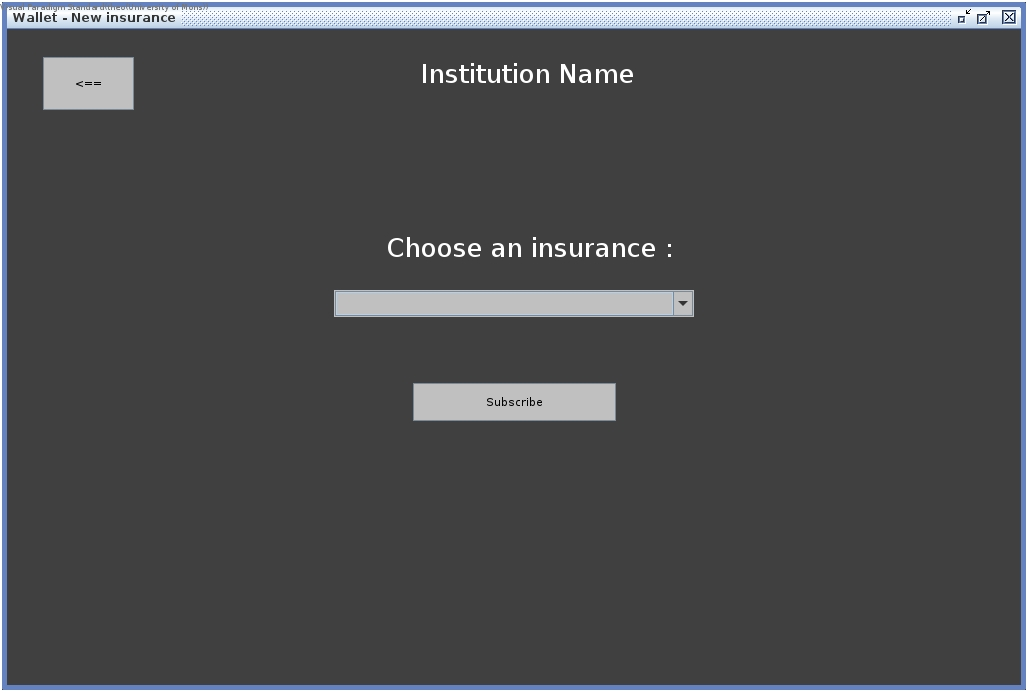
\includegraphics[scale=0.3]{ressources/photos_diagrammes/extensionThomas/gui1/addInsurance.jpg}
								\caption{Scène d'ajout d'une assurance}
						\end{figure} 
						Cette scène est la scène où l'on souscrit à une assurance elle est accessible depuis la ProductListScene en cliquant
						sur le bouton "My Insurances" Cette scène est composée d'une combo box permettant à l'utilisateur de choisir l'assurance
						à laquelle il veut sourscrire ainsi qu'un boouton subscribe.
				\newpage
				\item{InsuranceMenuScene} 
						\begin{figure}[h!]
								\centering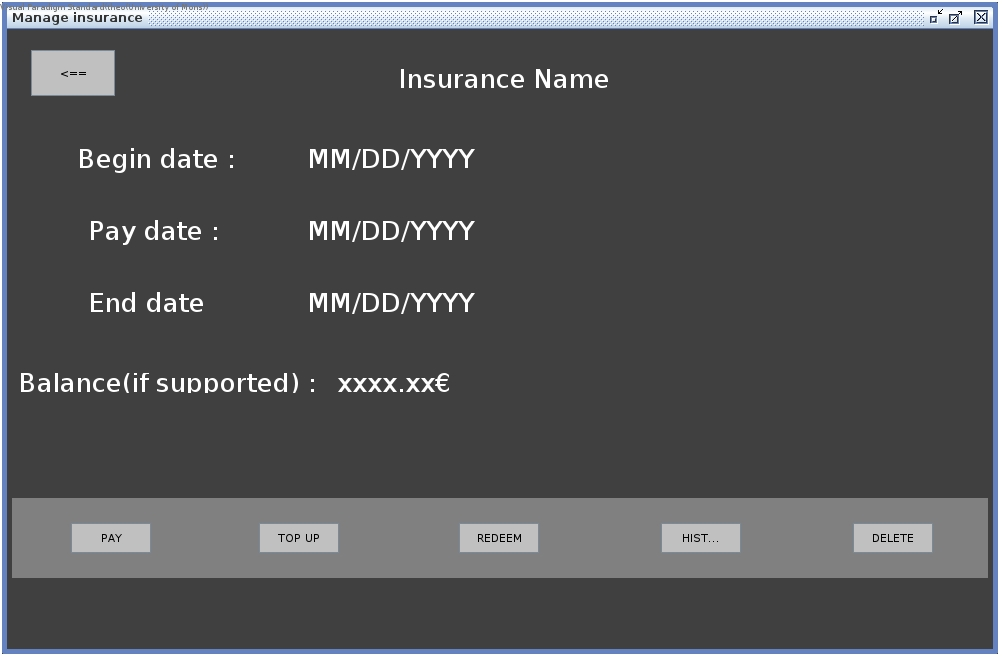
\includegraphics[scale=0.3]{ressources/photos_diagrammes/extensionThomas/gui1/insuranceMenu.jpg}
								\caption{Scène du menu d'une assurance}
						\end{figure}

						Cette correspond au menu d'une assurance. Toutes les informations pratiques de l'assurance y sont affichées ainsi que 
						les actions que l'on peut effectuer sur celle-ci. Ell est accessible depuis l'InsuranceListScene en cliquant sur un bouton 
						lié à une assurance. 

						\medskip

						Dans cette scène on retrouve 5 boutons. 3 permettant d'effectuer des transactions (PAY, TOP UP et REDEEM) ainsi qu'un bouton
						pour accéder à l'historique des transactions "HISTORY" et un bouton permettant de supprimer l'assurance "DELETE". 
				\newpage
				\item{InsuranceListScene} 
						\begin{figure}[h!]
								\centering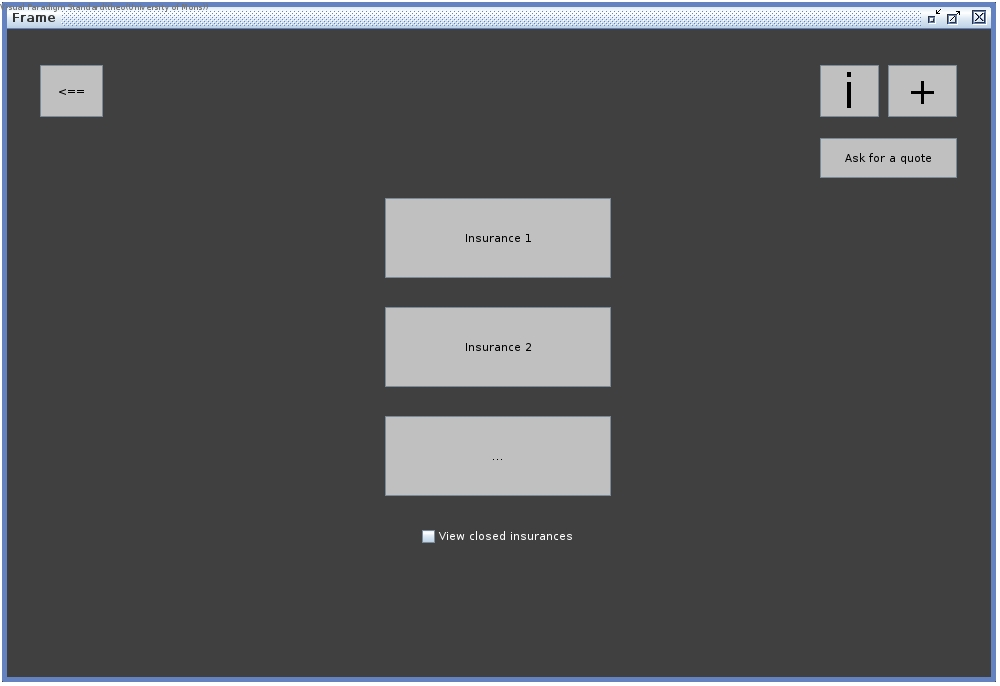
\includegraphics[scale=0.3]{ressources/photos_diagrammes/extensionThomas/gui1/insurancesList.jpg}
								\caption{Scène de la liste des assurances}
						\end{figure}

						Cette scène affiche la liste des assurances d'un client avec une check box "View closed insurances" permettant au client de voir 
						les assurances qu'il a supprimé. Elle contient également les différentes assurances qui sont cliquable et redirige vers la 
						InsuranceMenuScene. 
						Il y a également un bouton "+" permettant de rajouter une nouvelle assurance et envoyant sur la NewInsuranceScene.
						Il y un bouton "Ask for a quote" permettant de demander un devis et un bouton information "I" permettant d'obtenir des informations
						sur les assurances.
						\newpage
				\item{RedeemScene} 
						\begin{figure}[h!]
								\centering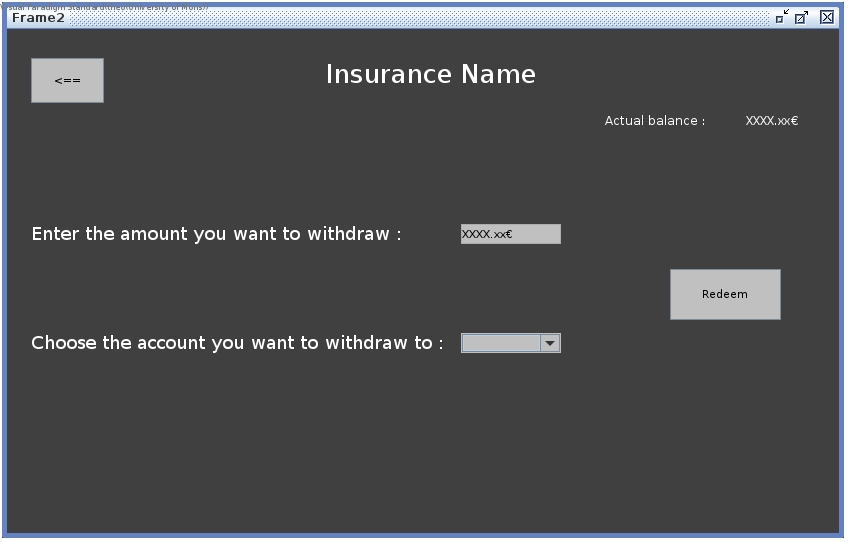
\includegraphics[scale=0.3]{ressources/photos_diagrammes/extensionThomas/gui1/redeemInsurance.jpg}
								\caption{Scène du retrait d'argent d'une assurance}
						\end{figure}
						Cette scène affiche la demande de retrait d'argent il y a 1 textfield permettant d'entrer le montant à retirer et une combo box 
						permettant de choisir le compte sur lequel on veut retier l'argent. Il y a un bouton "Redeem" permettant d'effectuer l'opération
						et un label affichant le solde actuel de l'assurance
						\newpage
				\item{TopUp Scene} 
						\begin{figure}[h!]
								\centering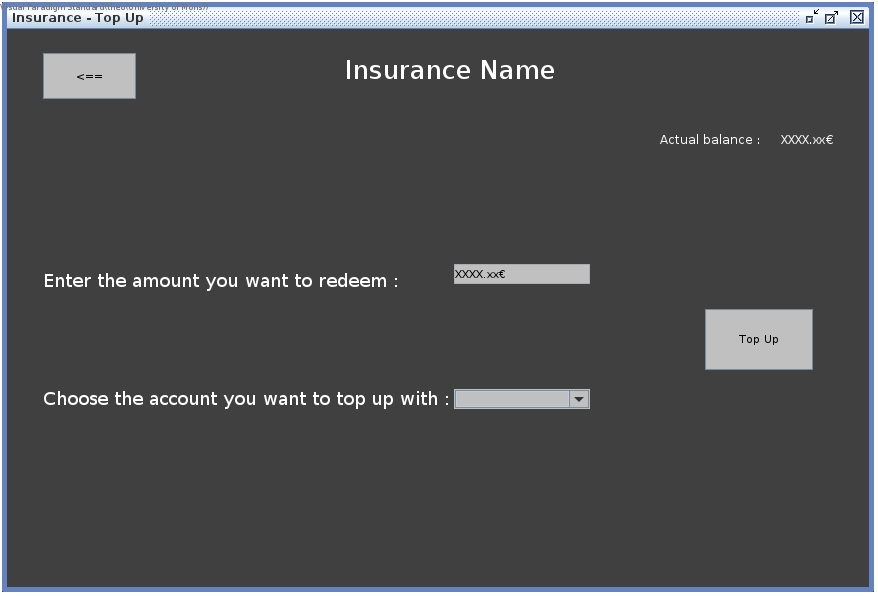
\includegraphics[scale=0.3]{ressources/photos_diagrammes/extensionThomas/gui1/topUpInsurance.jpg}
								\caption{Scène d'ajout d'argent d'une assurance}

								Cette scène fonctionne à peu de choses près comme la précédente. La scène PayScene n'a pas été représentée car jugée 
								trop similaires à ces deux-ci.
						\end{figure}
		\end{enumerate}
		\newpage

		\subsubsection{Application 2}
		\begin{enumerate}
		\item{ClientsMenuScene} 
						\begin{figure}[h!]
								\centering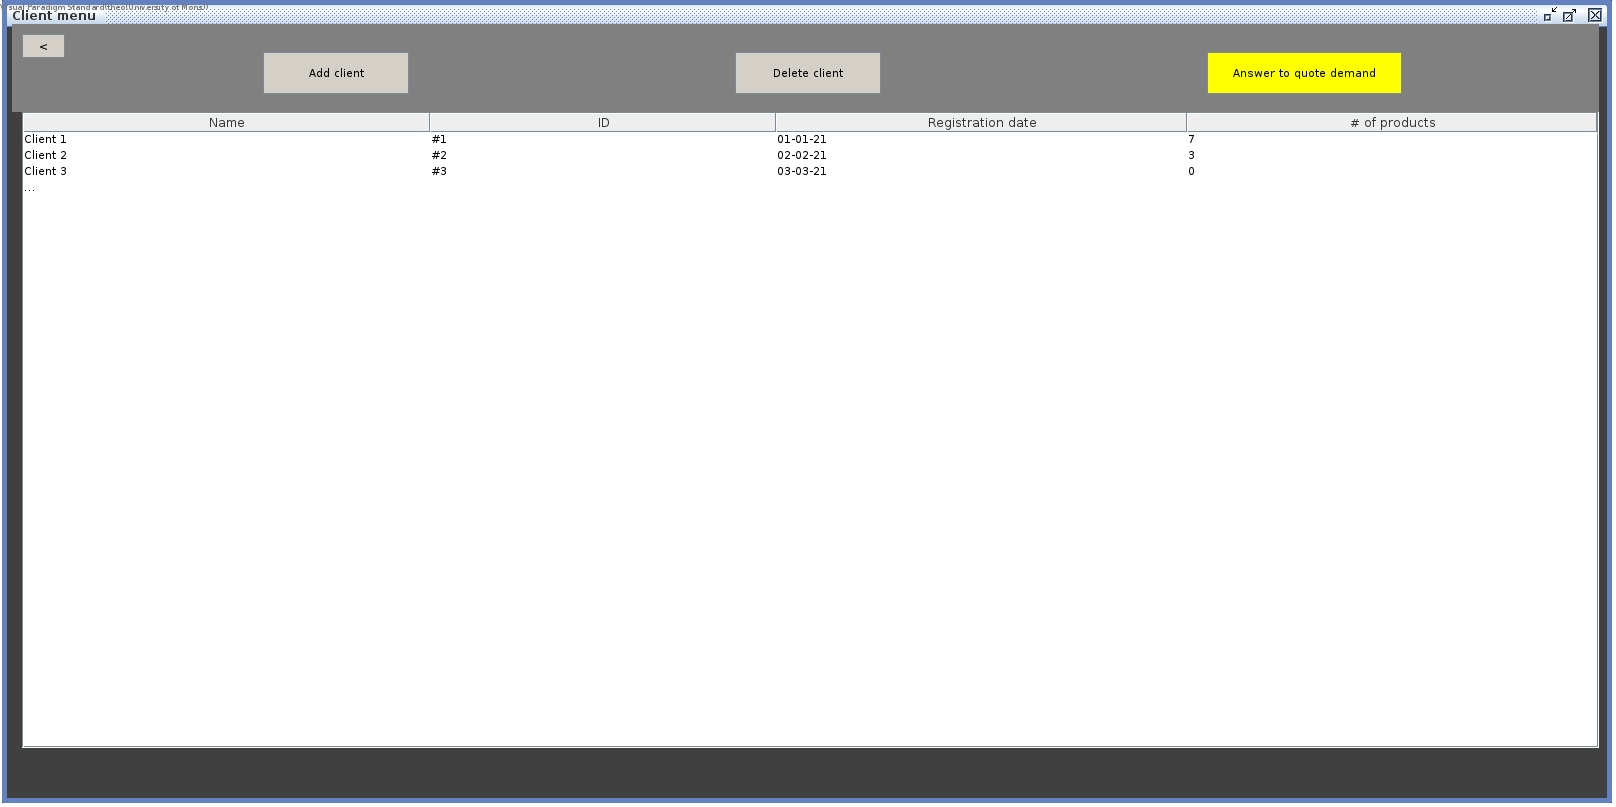
\includegraphics[scale=0.2]{ressources/photos_diagrammes/extensionThomas/gui2/clientsMenuScene.jpg}
								\caption{Scène du menu des clients}
						\end{figure}

						Cette rajoute uniquement un bouton "Answer to a quote demand" permettant d'accéder à la scène de réponse aux devis.
		\newpage
		\item{QuoteAnswerScene}
						\begin{figure}[h!]
								\centering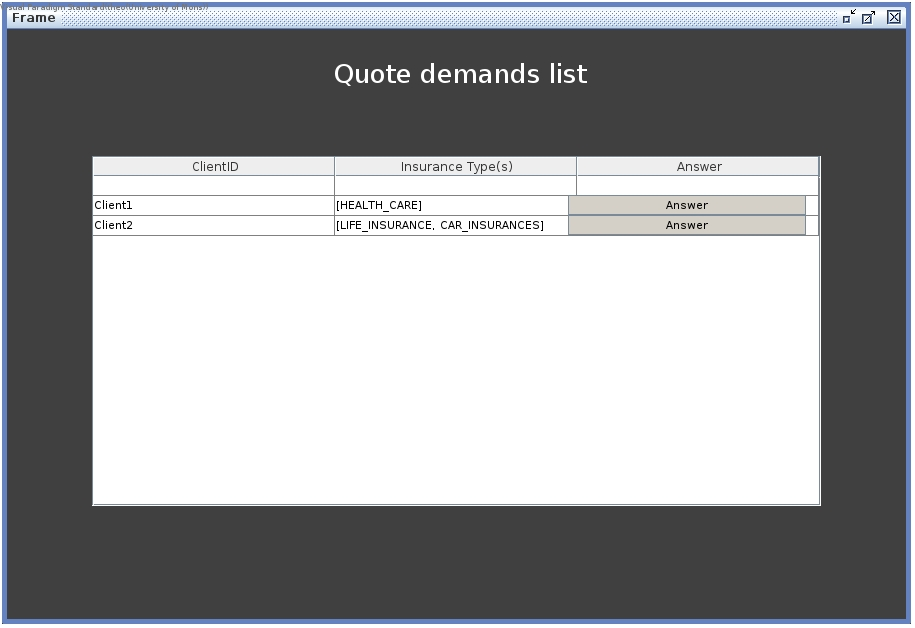
\includegraphics[scale=0.4]{ressources/photos_diagrammes/extensionThomas/gui2/quoteAnswerScene.jpg}
								\caption{Scène de réponse de demande à un devis}
						\end{figure}

						Cette affiche un tableau contenant les demandes des clients et un bouton "Answer" à coté de chaque afin d'envoyer la réponse au client.
		\end{enumerate}
\newpage
\end{document}
